\chapter{EFT-Modell mit MadGraph5}
In diesem Kapitel erfolgt eine Variation der Wilson-Koeffizienten mit Hilfe  von MadGraph5 unter der Verwendung eines EFT Modells. Dies ermöglicht die Berechnung eines approximierten Modells der Wirkungsquerschnitte für den EFTfitter mit dessen Hilfe später die Wilson-Koeffizienten bestimmt werden können. Dieses Modell wird benötigt, um die Laufzeiten des EFT-Fitters zu verringern.

\section{Zusammensetzung des Wirkungsquerschnitts}
Der Fit des EFTfitters basiert auf einem funktionellen Zusammenhang zwischen den Observablen, in diesem Fall den Wirkungsquerschnitten, und den Operatoren höherer Ordnung. Diese Abhängigkeit wird durch das implementierte Modell in der Likelihood ausgedrückt. Diese Likelihood wird mit einer Approximation durch MG bestimmt, da die Laufzeit des EFTfitters dadurch deutlich geringer wird.\\
Für die Berechnung des Wirkungsquerschnitts werden die zugehörigen Feynman-Graphen, sowohl die des SM, als auch die der EFT-Operatoren, betrachtet. Damit ergibt sich die Approximation des Wirkungsquerschnittes zu:
\begin{align}
  \sigma = \sigma_{SM} + \frac{1}{\Lambda^2} \sum_{i} C_i \sigma_i^\text{interf.} + \frac{1}{\Lambda^4} \sum_{i \leq j} C_i C_j \sigma_{ij}^\text{BSM} + \mathcal{O} \left(\frac{1}{\Lambda^6}\right).
\end{align}
Die einzelnen Wirkungsquerschnitte $\sigma$ besitzen eine quadratische Abhängigkeit von den Wilson-Koeffizienten $C_i$ und die BSM-Beiträge in führender Ordnung ergeben sich durch die Interferenz zwischen dem SM und der BSM-Physik. Dies liegt unter Anderem daran, dass die Beiträge durch die Interferenz zwischen den BSM-Physik-Beiträgen untereinander mit $\frac{1}{\Lambda^4}$ unterdrückt sind. Untersuchungen\cite{Wilson-Beiträge} haben ergeben, dass diese Beiträge trotzdem betrachtet werden sollten, um ein Modell für die Abhängigkeit der Wirkungsquerschnitte von den Wilson-Koeffizienten zu erhalten, da sie deutlich zur Genauigkeit von diesem beitragen.

\section{Variation der Wilson-Koeffizienten mit MadGraph5}%
%
Zur Bestimmung des Modells ist es notwendig die Wirkungsquerschnitte für verschiedene Konfigurationen der Wilson-Koeffizienten zu bestimmen, um sowohl den Einfluss einzelner als auch mehrerer Operatoren untersuchen zu können.
Eine Möglichkeit die Wilson-Koeffizienten zu variieren, ist mit Hilfe eines  EFT-Modells für MG, das Operatoren der Massendimension sechs enthält und damit eine Berechnung der Wirkungsquerschnitte unter dem Einfluss dieser ermöglicht. Dazu wird in MG das TEFT\_EF UFO Modell\cite{EFTModell} eingebunden.
Dies enthält einige der für die Top-Quark-Physik relevanten Operatoren der Dimension sechs und insbesondere die, die an dem Prozess $pp~\rightarrow~t\bar{t}~\gamma$ beteiligt sind.
Die Berechnung erfolgt mit dem genannten Modell in NLO in QCD unter der Verwendung des $\text{CTEQ}6\text{L}1$ PDF-Sets.
Zudem wird die BSM-Energieskala auf $\Lambda = \SI{1}{\tera\electronvolt}$ festgelegt.
Unter diesen Vorraussetzungen wird der Prozess $pp~\rightarrow~t\bar{t}~\gamma$ mit den von ATLAS genutzten Schnitten für den gemessenen Phasenraum implementiert.\\
Die berechneten Monte Carlo Wirkungsquerschnitte:
\begin{align}
  \sigma_{MC}({C_i}) = \sigma_{SM} + \sum_{i} C_i \frac{\sigma_i}{\Lambda^2} + \sum_{i \leq j} C_i C_j \frac{\sigma_{ij}}{\Lambda^4} + \mathcal{O}\left(\frac{1}{\Lambda^6}\right)
\end{align}
bilden die Stützstellen zur späteren Bestimmung der gesuchten Parameter $\sigma_i$ und $\sigma_{ij}$.
Mit Hilfe des Vakuumerwartungswerts des Higgs $v = \SI{246}{\giga\electronvolt}$ und der Wahl $\Lambda = \SI{1}{\tera\electronvolt}$ lassen sich die $\sigma_{MC}$ in die Größenordnung einer Kopplungsstärke umrechnen.
Unter Vernachlässigung von Termen der Ordnung $\mathcal{O}(\frac{1}{\Lambda^6})$, ergeben sie sich zu:
\begin{align}
  \sigma_{MC}({\tilde{C_i}}) \approx \bar{\sigma}_{SM} + \sum_{i} \tilde{C_i} \bar{\sigma_i} + \sum_{i \leq j} \tilde{C_i} \tilde{C_j} \bar{\sigma}_{ij}.
\end{align}
Hierbei sind die $\tilde{C}_i = \frac{v^2}{\Lambda^2} C_i$ und $\bar{\sigma}_i$ die zugehörgen Parameter.
Bei der Berechnung des $t\bar{t}\gamma$ Produktionswirkungsquerschnitts können, wie in Kapitel~\ref{top} bereits erwähnt, die Operatoren $O_{tG}$, $O_{tW}$ und $O_{tB}$ beitragen. Damit ergibt sich die Interpolationsfunktion zu:
\begin{align}
  \sigma_{t\bar{t}\gamma, MC}({\tilde{C}_{tG}, \tilde{C}_{tW}, \tilde{C}_{tB}}) = \bar{\sigma}_{SM} + \tilde{C}_{tG}\bar{\sigma}_{tG} + \tilde{C}_{tW}\bar{\sigma}_{tW} + \tilde{C}_{tB}\bar{\sigma}_{tB}\\ \nonumber
  + \tilde{C}_{tG}^2\bar{\sigma}_{tGtG} + \tilde{C}_{tW}^2\bar{\sigma}_{tWtW} + \tilde{C}_{tB}^2\bar{\sigma}_{tBtB}\\
  + \tilde{C}_{tG} \tilde{C}_{tW}\bar{\sigma}_{tGtW} + \tilde{C}_{tG} \tilde{C}_{tB}\bar{\sigma}_{tGtB} + \tilde{C}_{tW} \tilde{C}_{tB}\bar{\sigma}_{tWtB} \nonumber
\end{align}
und es müssen insgesamt zehn Parameter $\bar{\sigma_i}$ und $\bar{\sigma}_{ij}$ bestimmt werden. Dazu werden die Wilson-Koeffizienten $C_{tG}$, $C_{tW}$ und $C_tB$ im Bereich $[-30~,~30]$ variiert. Auf Grund der statistischen Unsicherheiten werden insgesamt $50$ verschiedene Variationen durchgeführt, bei denen ein, zwei oder alle der Wilson-Koeffizienten ungleich Null sind.
Um erneut nur die semileptonischen Endzustände zu betrachten, müssen auch in diesem Fall die $\sigma_{t\bar{t}\gamma, MC}$ mit dem semileptonischen Verzweigungsverhältnis $\mathrm{BR} = \SI{30}{\percent}$ multipliziert werden.
Aus diesen Berechnungen lassen sich dann mit der Methode der kleinsten Quadrate die gesuchten Parameter bestimmen, aus denen sich schließlich das Modell für den EFTfitter ergibt.


\section{Ergebnisse des Fits zur Bestimmung des Modells für den EFTfitter}
\label{Modell}
Durch die Bestimmung der gesuchten Parameter mit der Methode der kleinsten Quadrate werden die folgenden Wirkungsquerschnitte bestimmt:
\begin{table}[H]
    \centering
   \begin{tabular}{ll}
     $\bar{\sigma}_{SM}   = 202.19 $  & $\bar{\sigma}_{tW}   = 21.68$\\
     $\bar{\sigma}_{tB}   = 21.69$    & $\bar{\sigma}_{tG}   = 761.42$\\
     $\bar{\sigma}_{tWtW} = 11.7 $    & $\bar{\sigma}_{tBtB} = 11.77$\\
     $\bar{\sigma}_{tGtG} = 48.44$    & $\bar{\sigma}_{tGtW} = 6863.76$\\
     $\bar{\sigma}_{tGtB} = -6483.31$ & $\bar{\sigma}_{tWtB} = 279.22$
   \end{tabular}
\end{table}
Die Unsicherheiten aus dem Fit mit der Methode der kleinsten Quadrate werden hier vernachlässigt, da diese nicht im Modell des EFTfitters implementiert werden können.\\
In den gezeigten Abbildungen~\ref{fig:tp} und~\ref{fig:WtG} ist erkennbar, dass der Fit die erwartete quadratische Form in den jeweiligen Parametern aufweist.
Die für die beiden Wilson-Koeffizienten $\tilde{C}_{tW}$ und $\tilde{C}_{tB}$ berechneten Wirkungsquerschnitte folgen ziemlich genau diesem parabelförmigen Verlauf.
Zudem stimmen die Wirkungsquerschnitte und damit der Verlauf nahezu überein; dies ist in Abbildung~\ref{fig:WtW} und~\ref{fig:WtB} veranschaulicht. Da die beiden Wilson-Koeffizienten zu den beiden an der Photonabstrahlung beteiligten Operatoren gehören, war zu erwarten, dass beide ähnliche Ergebnisse liefern. Lediglich die berechneten Wirkungsquerschnitte für den Wilson-Koeffizienten $\tilde{C}_{tG}$ weisen teilweise Abweichungen auf, wie in Abbildung~\ref{fig:WtG} erkennbar.\\
Dies könnte daran liegen, dass der Wertebereich der berechneten Wirkungsquerschnitte deutlich größer ist. Dadurch sind größere Abweichung plausibel, die ebenfalls größere Unsicherheiten mit sich bringen. Die Abweichungen könnten verbessert werden, indem zum einen mehr Stützstellen berechnet werden und zum anderen genauere Monte Carlo Rechnungen erfolgen.\\
\begin{figure}
  \begin{subfigure}[c]{0.5\textwidth}
    \centering
    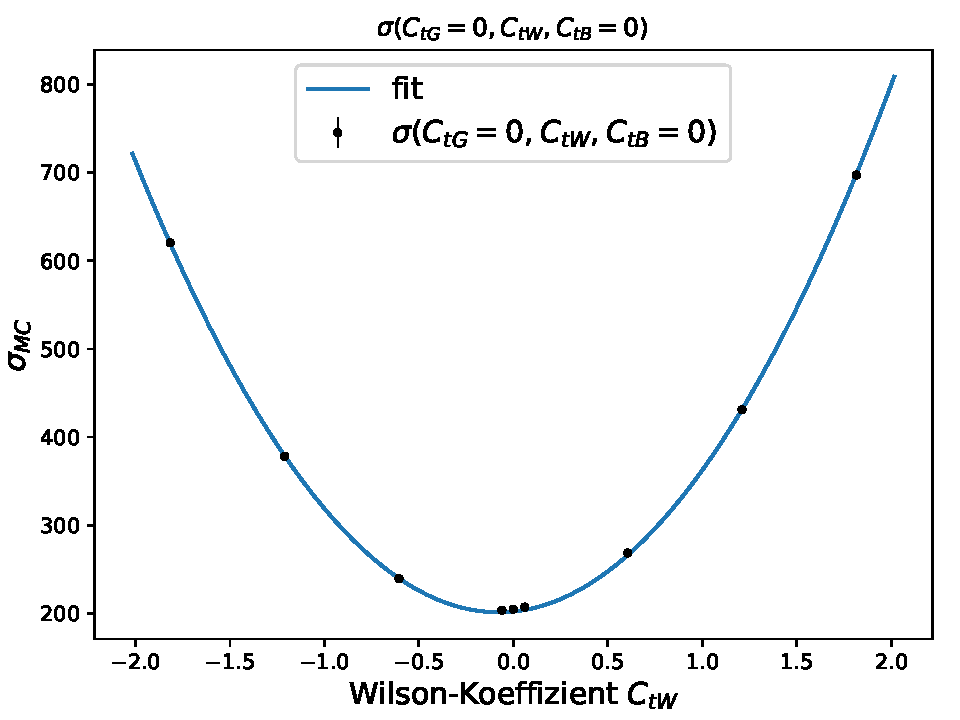
\includegraphics[width=\textwidth]{Plots/combi_plot_tW.pdf}
    \subcaption{Verlauf für $\tilde{C}_{tW}$ mit $\tilde{C}_{tB}=\tilde{C}_{tG}=0$.}
    \label{fig:WtW}
  \end{subfigure}
  \begin{subfigure}[c]{0.5\textwidth}
    \centering
    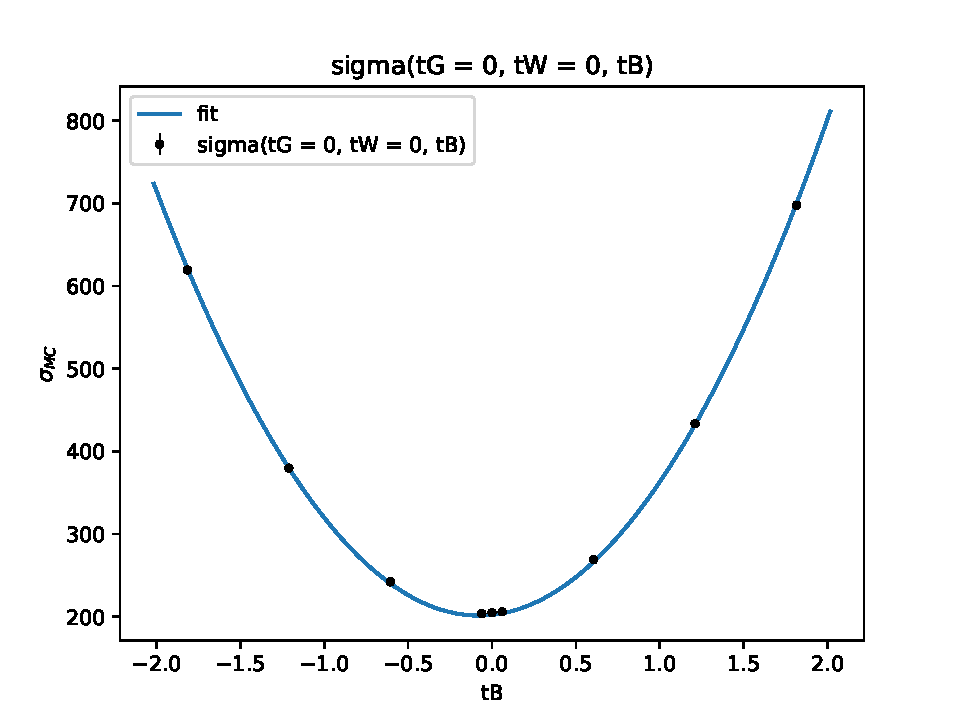
\includegraphics[width=\textwidth]{Plots/combi_plot_tB.pdf}
    \subcaption{Verlauf für $\tilde{C}_{tB}$ mit $\tilde{C}_{tW}=\tilde{C}_{tG}=0$.}
    \label{fig:WtB}
  \end{subfigure}
  \caption{Graphische Darstellung des parabelförmigen Verlaufs der Wirkungsquerschnitte für die Betrachtung einzelner Wilson-Koeffizienten.}
  \label{fig:tp}
\end{figure}
\begin{figure}
  \centering
  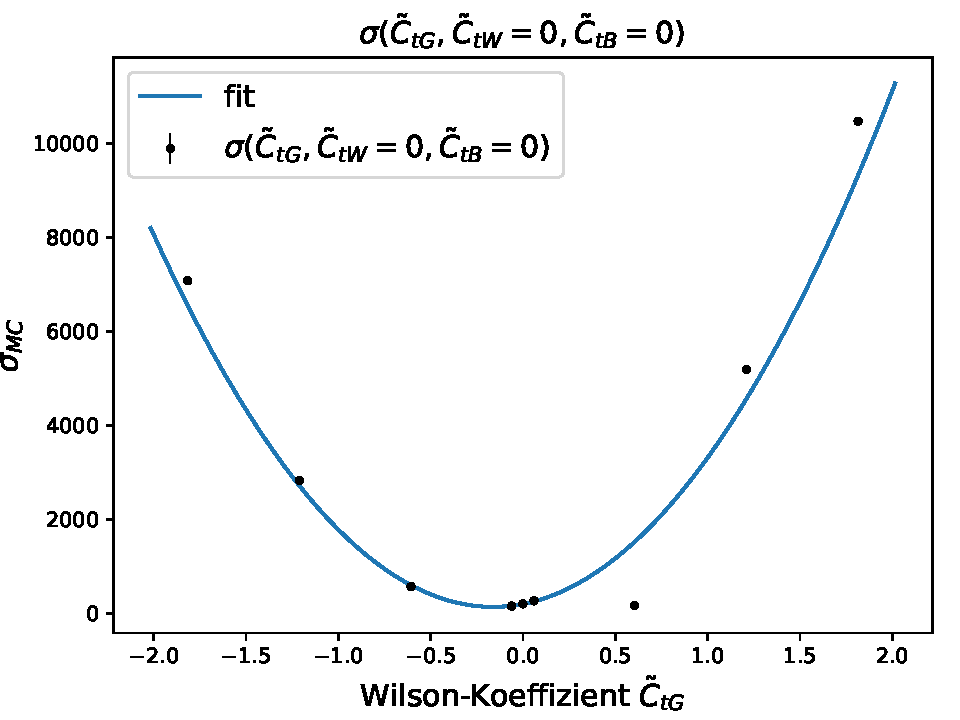
\includegraphics[width=0.6\textwidth]{Plots/combi_plot_tG.pdf}
  \caption{Graphische Darstellung des parabelförmigen Verlaufs der Wirkungsquerschnitte für den Wilson-Koeffizienten $\tilde{C}_{tG}$, wenn $\tilde{C}_{tW}=\tilde{C}_{tB}=0$ ist.}
  \label{fig:WtG}
\end{figure}
%
%
\chapter{EFT-Interpretation des \texorpdfstring {$t\bar{t}\gamma$}{math} Produktionswirkungsquerschnitts mit dem EFTfitter}
In diesem Kapitel erfolgt die Untersuchung der am $t\bar{t}\gamma$ Produktionswirkungsquerschnitt beteiligenten Wilson-Koeffizienten mit dem EFTfitter. Dazu wird das mit MadGraph bestimmte Modell aus Kapitel~\ref{Modell} im EFTfitter implemeniert und mit Hilfe der ATLAS Messung die Wilson-Koeffizienten eingeschränkt.

\section{Einschränkung der Wilson-Koeffizienten}
Mit Hilfe des EFTfitter kann der von ATLAS gemessene $t\bar{t}\gamma$ Produktionswirkungsquerschnitt auf mögliche Abweichungen durch die EFT-Operatoren $O_{tG}$, $O_{tW}$ und $O_{tB}$ getestet werden. Dazu wird das in Kapitel~\ref{Modell} berechnete Modell verwendet. Es ermöglicht Einschränkungen für die Wilson-Koeffizienten der EFT-Operatoren zu finden.\\
In den Abbildungen~\ref{fig:ctg},~\ref{fig:ctw} und~\ref{fig:ctb} sind die marginalisierten, eindimensionalen Posteriorverteilung der Wilson-Koeffizienten, die mit Hilfe des EFTfitters berechnet werden, dargestellt.
Da der Fit mit einem quadratischen Modell in den Wilson-Koeffizienten durchgeführt wird, stimmt die Messung an zwei Stellen mit der Vorhersage überein, sodass sich zwei Peaks ergeben.
Da für jeden Wilson-Koeffizienten eines der Maxima bei Null liegt und das kleinste $\SI{68.1}{\percent}$ Intervall diesen Wert umfasst, kann die SM Vorhersage, dass die Wilson-Koeffizienten Null sind, nicht verworfen werden.
Dieses Intervall ist für alle Wilson-Koeffizient in Abbildung~\ref{fig:wil} dargestellt. Auffällig ist, dass die Intervalle alle die Null enthalten, aber nur $\tilde{C}_{tG}$ um diese zentriert ist und zudem die Einschränkung deutlich kleiner ist.
Dies liegt an den größeren Abweichungen der Parameter von dem parabelförmigen Verlauf, die bereits in Abbildung~\ref{fig:WtG} beobachtet wurden.
Zudem ist zu beobachten, dass die Einschränkungen für $\tilde{C}_{tW}$ und $\tilde{C}_{tB}$ nahezu übereinstimmen.
Dies war zu erwarten, da beide Wilson-Koeffizienten aus der Photonabstrahlung stammen und somit direkt mit einander verbunden sind.
Die noch relativ großen Intervalle für die Einschränkung von $\tilde{C}_{tW}$ und $\tilde{C}_{tB}$ motivieren eine Kombination mit weiteren Observablen, die sensitiv auf die gleichen Operatoren sind. So kann eine bessere Einschränkung erfolgen und unter Umständen eines der beiden Maxima ausgeschlossen werden, sodass sich das $\SI{68.1}{\percent}$ Intervall verkleinert.
Um eine höhere Aussagekraft dieser Ergebnisse zu erhalten, empfielt es sich die Einschränkung mit mehreren Messungen für den $t\bar{t}\gamma$ Produktionswirkungsquerschnitt zu berechnen.
\begin{figure}
    \centering
    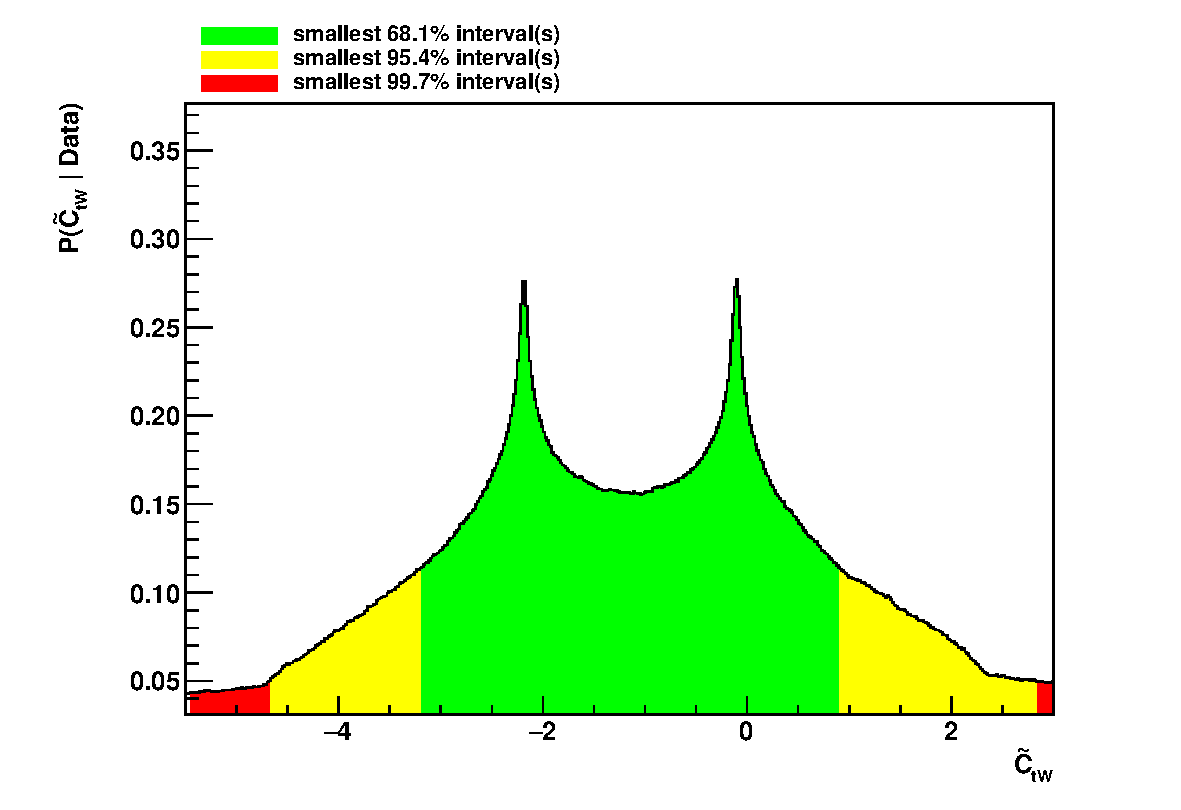
\includegraphics[width=0.8\textwidth]{Plots/ctw.pdf}
    \caption{Eindimensionale Posteriorverteilung des Wilson-Koeffizienten $\tilde{C}_{tW}$.}
    \label{fig:ctw}
\end{figure}
\begin{figure}
    \centering
    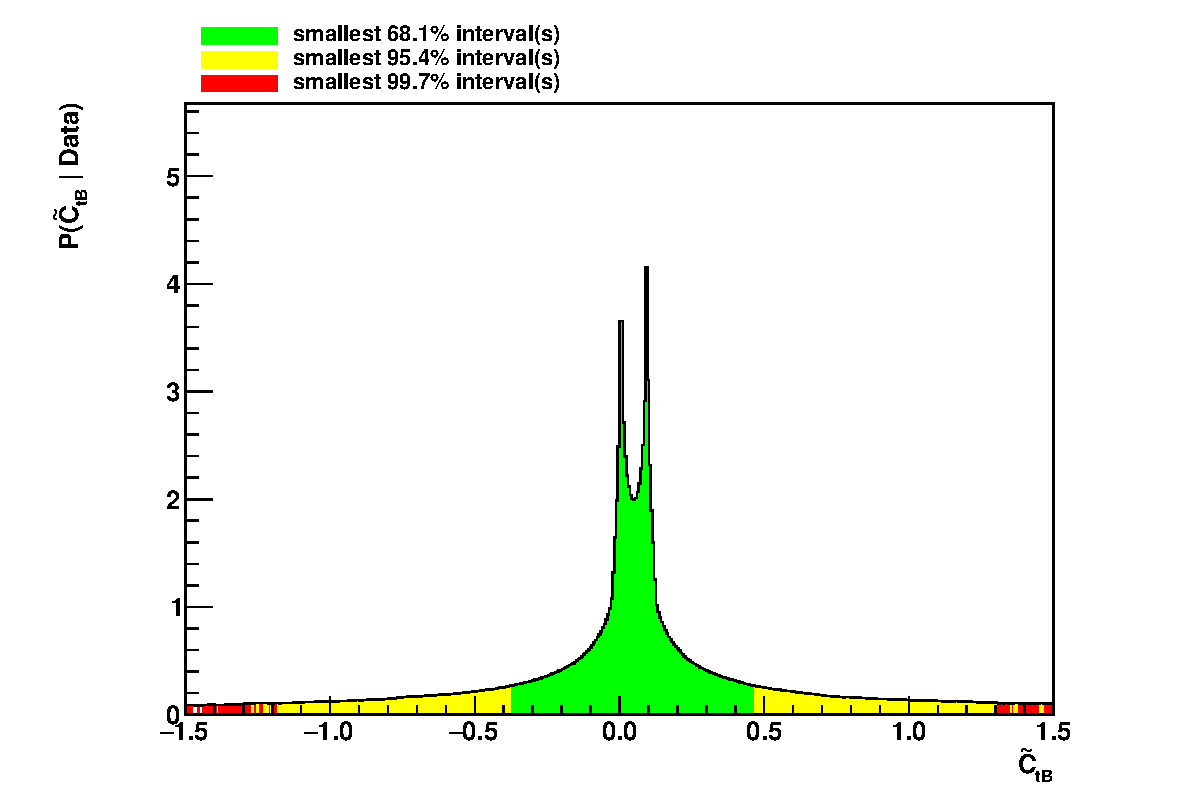
\includegraphics[width=0.8\textwidth]{Plots/ctb.pdf}
    \caption{Eindimensionale Posteriorverteilung des Wilson-Koeffizienten $\tilde{C}_{tB}$.}
    \label{fig:ctb}
\end{figure}
\begin{figure}
    \centering
    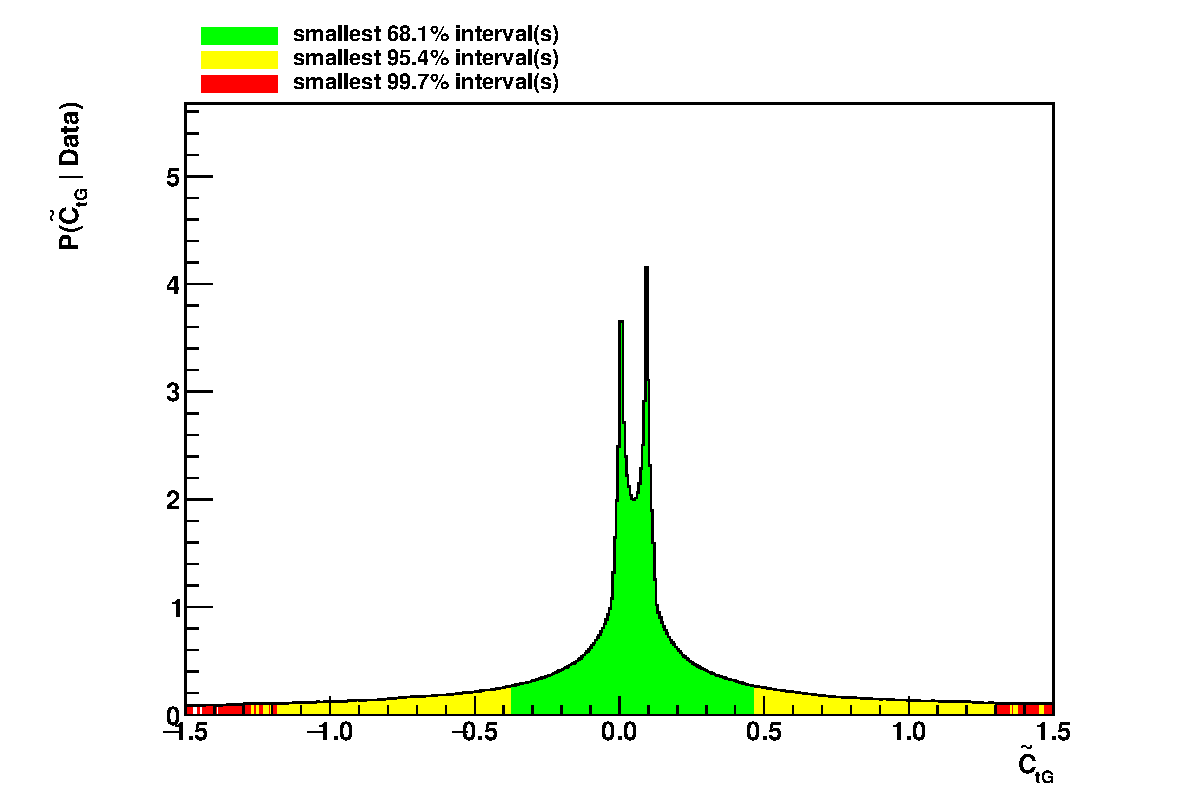
\includegraphics[width=0.8\textwidth]{Plots/ctg.pdf}
    \caption{Eindimensionale Posteriorverteilung des Wilson-Koeffizienten $\tilde{C}_{tG}$.}
    \label{fig:ctg}
\end{figure}
\begin{figure}
    \centering
    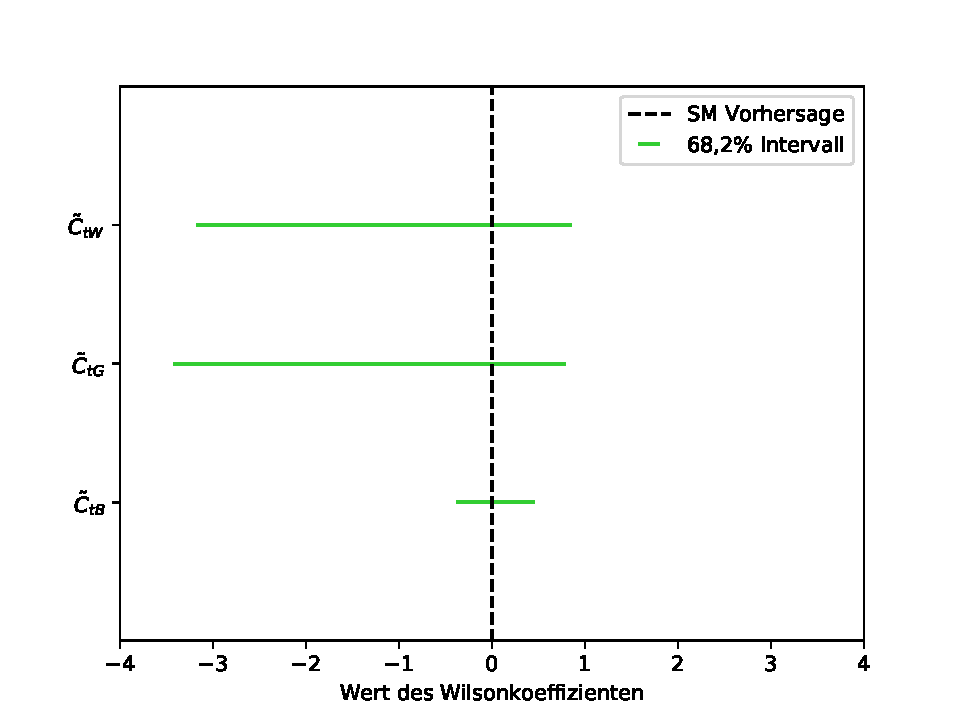
\includegraphics[width=0.7\textwidth]{Plots/wilson.pdf}
    \caption{Darstellung des kleinsten $\SI{68.1}{\percent}$ Intervalls der Wilson-Koeffizienten zur Veranschaulichung der Verträglichkeit mit Null.}
    \label{fig:wil}
\end{figure}
%
%
\chapter{Zusammenfassung}
Um eine Kombination der in unterschiedlichen Phasenräumen erfolgten Messungen des $t\bar{t}\gamma$ Produktionswirkungsquerschnitts zu ermöglichen, ist zunächst eine Phasenraumstudie mit MadGraph5 erfolgt. Hierzu wurde zunächst, sowohl für die ATLAS Messung als auch für die beiden CMS-Messungen ein $k$-Faktor als Näherung zwischen der LO und NLO Rechnung bestimmt. Unter Anwendung dieses Faktor lässt sich der Phasenraumfaktor zwischen den beiden gemessenen Phasenräumen zu $f=3$ bestimmen. Erweitert man die CMS Messungen um diesen Faktor in den ATLAS Phasenraum ergeben sie sich zu:
\begin{align*}
  \sigma^{fid(A), \text{CMS}}_{t\bar{t}\gamma, e} &= 410 \pm 140~ \si{\femto\barn}\\
  \sigma^{fid(A), \text{CMS}}_{t\bar{t}\gamma, \mu} &= 350 \pm 100~ \si{\femto\barn}.
\end{align*}
Im Anschluss erfolgt eine einfache Kombination der Messungen mit dem EFTfitter unter der Annahme, dass sie unkorreliert sind. Der kombinierte Produktionswirkungsquerschnitt ergibt:
\begin{align*}
  \sigma_{\text{Kombi}} = 149,79 \pm 17,57~ \si{\femto\barn}.
\end{align*}
Es fällt auf, dass das kombinierte Ergebnis sehr nahe an der ATLAS Messung liegt, dies liegt unter anderem daran, dass Gewichtung der Messung in der Kombination anhand ihrer Fehler erfolgt. Diese sind durch die Erweiterung bei den CMS Messungen sehr groß. Daher empfielt es sich weiter Studien zu den Unsicherheiten und ihren Gültigkeiten in den einzelnen Phasenräumen durchzuführen. Die anschließend für die Kombination durchgeführte Korrelationsstudie ergibt, dass die Kombination für eine Korrelation zwischen den CMS Messungen nahezu unabhängig ist, sodass in diesem Fall eine unkorrelierte Annahme zu rechtfertigen ist. Jedoch weißt die Kombination für eine Korrelation zwischen den CMS Messungen und der ATLAS Messung eine starke Abhängigkeit auf. Dies motiviert neben der genaueren Untersuchung der Unsicherheiten, auch die Korrelation zwischen den Messungen zu bestimmen.\\
Da der kombinierte Wert nahe der ATLAS Messung liegt, wird für die EFT-Interpretation nur noch diese verwendet. Da der EFTfitter für eine genaue Rechnung eine extrem hohe Laufzeit besitzt, erfolgt zunächst die Bestimmung eines Modells zur Approximation mit Hilfe von MadGraph. Dieses Modell wird anschließend im EFTfitter implementiert, um mit ihm die am $t\bar{t}\gamma$ Produktionswirkungsquerschnitt beteiligten Wilson-Koeffizienten $C_{tG}$, $C_{tW}$ und $C_{tB}$ einzugrenzen. Dabei ergibt sich für alle drei Koeffizienten eine Verträglichkeit des kleinsten $\SI{68.1}{\percent}$ Intervalls mit der Null. Die Intervalle sind jedoch für die an der Photonabstrahlung beteiligten Wilson-Koeffizienten $C_{tW}$ und $C_{tB}$ relativ breit, sodass eine weiter Untersuchung anzustreben ist.
